\documentclass{article}%
\usepackage[T1]{fontenc}%
\usepackage[utf8]{inputenc}%
\usepackage{lmodern}%
\usepackage{textcomp}%
\usepackage{lastpage}%
\usepackage[head=40pt,margin=0.5in,bottom=0.6in]{geometry}%
\usepackage{graphicx}%
%
\title{\textbf{Así fue hallado el cadáver de Fernando Albán}}%
\author{El Nacional Web}%
\date{08/10/2018}%
%
\begin{document}%
\normalsize%
\maketitle%
\textbf{URL: }%
http://www.el{-}nacional.com/noticias/sucesos/asi{-}fue{-}hallado{-}presunto{-}cadaver{-}fernando{-}alban\_254883\newline%
%
\textbf{Periodico: }%
EN, %
ID: %
254883, %
Seccion: %
Sucesos\newline%
%
\textbf{Palabras Claves: }%
Sebin, Sucesos\newline%
%
\textbf{Derecho: }%
1.1%
, Otros Derechos: %
1.2, 1.10%
, Sub Derechos: %
1.1.1.3, 1.2.2, 1.10.1.1%
\newline%
%
\textbf{EP: }%
NO\newline%
\newline%
%
\textbf{\textit{El concejal se encontraba detenido en la sede del Sebin en Plaza Venezuela desde este viernes~}}%
\newline%
\newline%
%
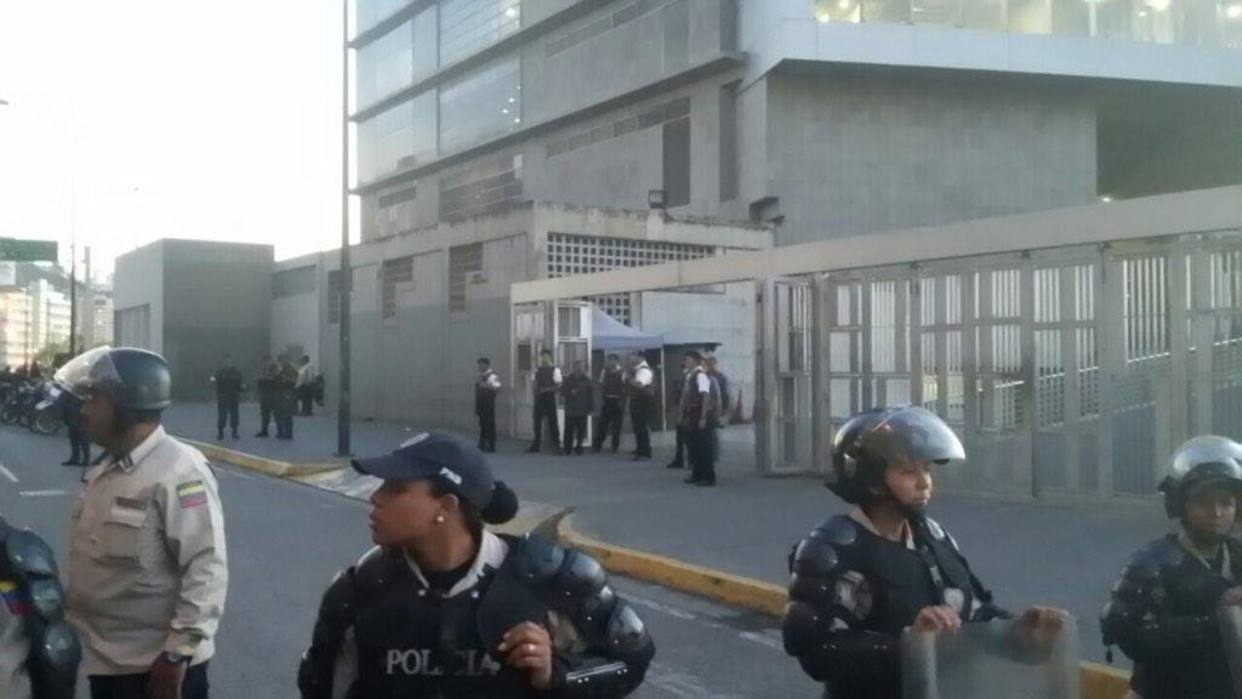
\includegraphics[width=300px]{255.jpg}%
\newline%
%
El concejal del municipio Libertador, Fernando~Albán, fue hallado sin vida~en la sede del Servicio Bolivariano de Inteligencia Nacional ubicado en Plaza Venezuela.%
\newline%
%
Tarek William Saab, fiscal general designado por la asamblea nacional contituyente, informó que el cuerpo de Albán fue hallado sin vida en las adyacencias del ente. Saab informó que el concejal pidió~presuntamente permiso para ir al baño cuando se lanzó de la ventana de un décimo piso.%
\newline%
%
Albán se encontraba detenido desde este viernes en el aeropuerto Internacional Simón Bolívar por funcionarios del Sebin. Néstor Reverol, ministro de Interior, Justicia y Paz, aseguró que se designó una comisión del Ministerio Público para investigar~la muerte de Albán.%
\newline%
%
\end{document}